% !TEX root = main.tex

%%%%%%%%%%%%%%%%%%%%%%%%%%%%%%%%%%%%%%%%%%%%%%%%%%%%%%%%%%%%%%%%%%%%%%%%%%%%%%%%%%%%%%%%%%%%%%%%
\section{結果}
%%%%%%%%%%%%%%%%%%%%%%%%%%%%%%%%%%%%%%%%%%%%%%%%%%%%%%%%%%%%%%%%%%%%%%%%%%%%%%%%%%%%%%%%%%%%%%%%

\subsection{実験課題1}
シミュレーション結果を以下の図1に示す.$x$座標が正の電極板に$10\,[\si{\volt}]$
の印加電圧がかかっており,$x$座標が負の電極板はGNDに接続しているとする.
\begin{figure}[H]
    \begin{center}
        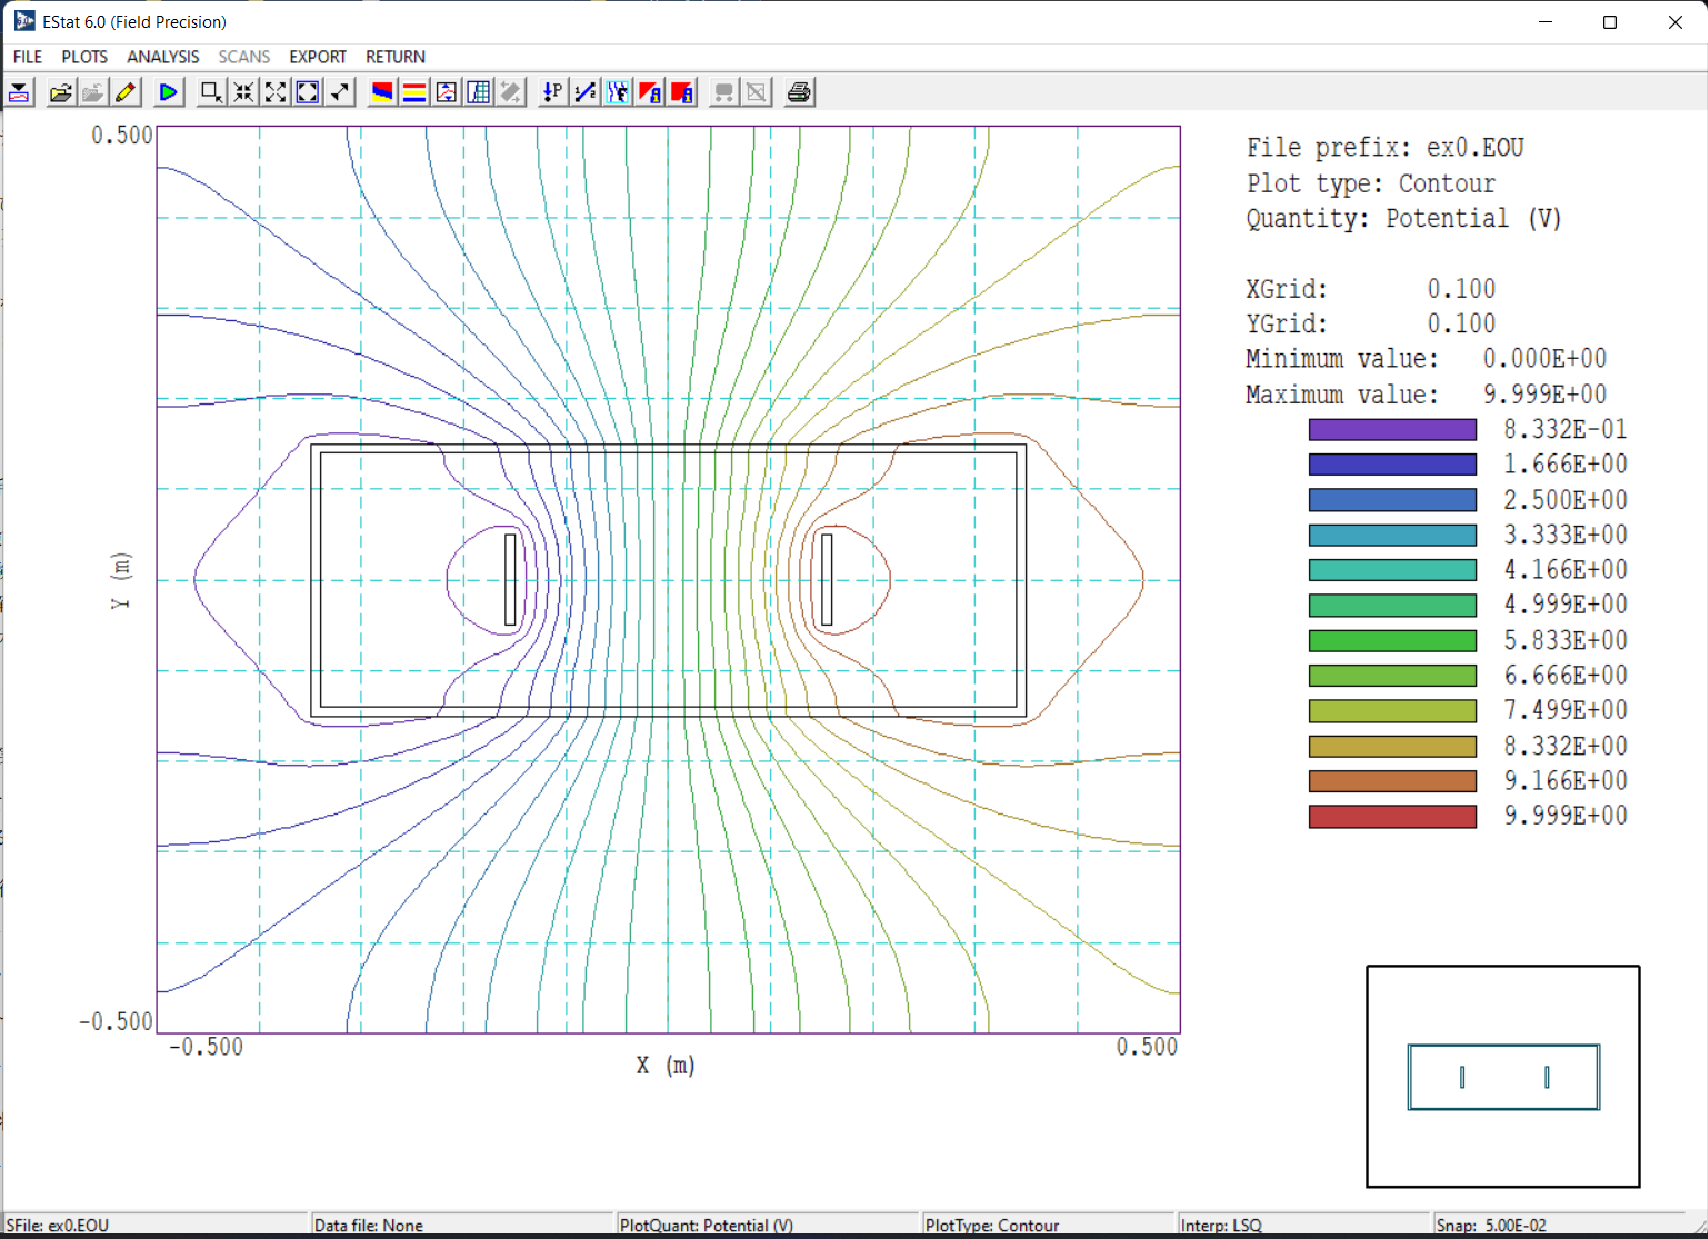
\includegraphics[scale=0.5]{figure1.pdf}
        \caption{第1週目の実験時のセットアップにおける等電位面}
    \end{center}
\end{figure}
\newpage

\subsection{実験課題2}
シミュレーション結果を以下の図2に示す.$x$座標が正の電極板に$10\,[\si{\volt}]$
の印加電圧がかかっており,$x$座標が負の電極板はGNDに接続しているとする.
\begin{figure}[H]
    \begin{center}
        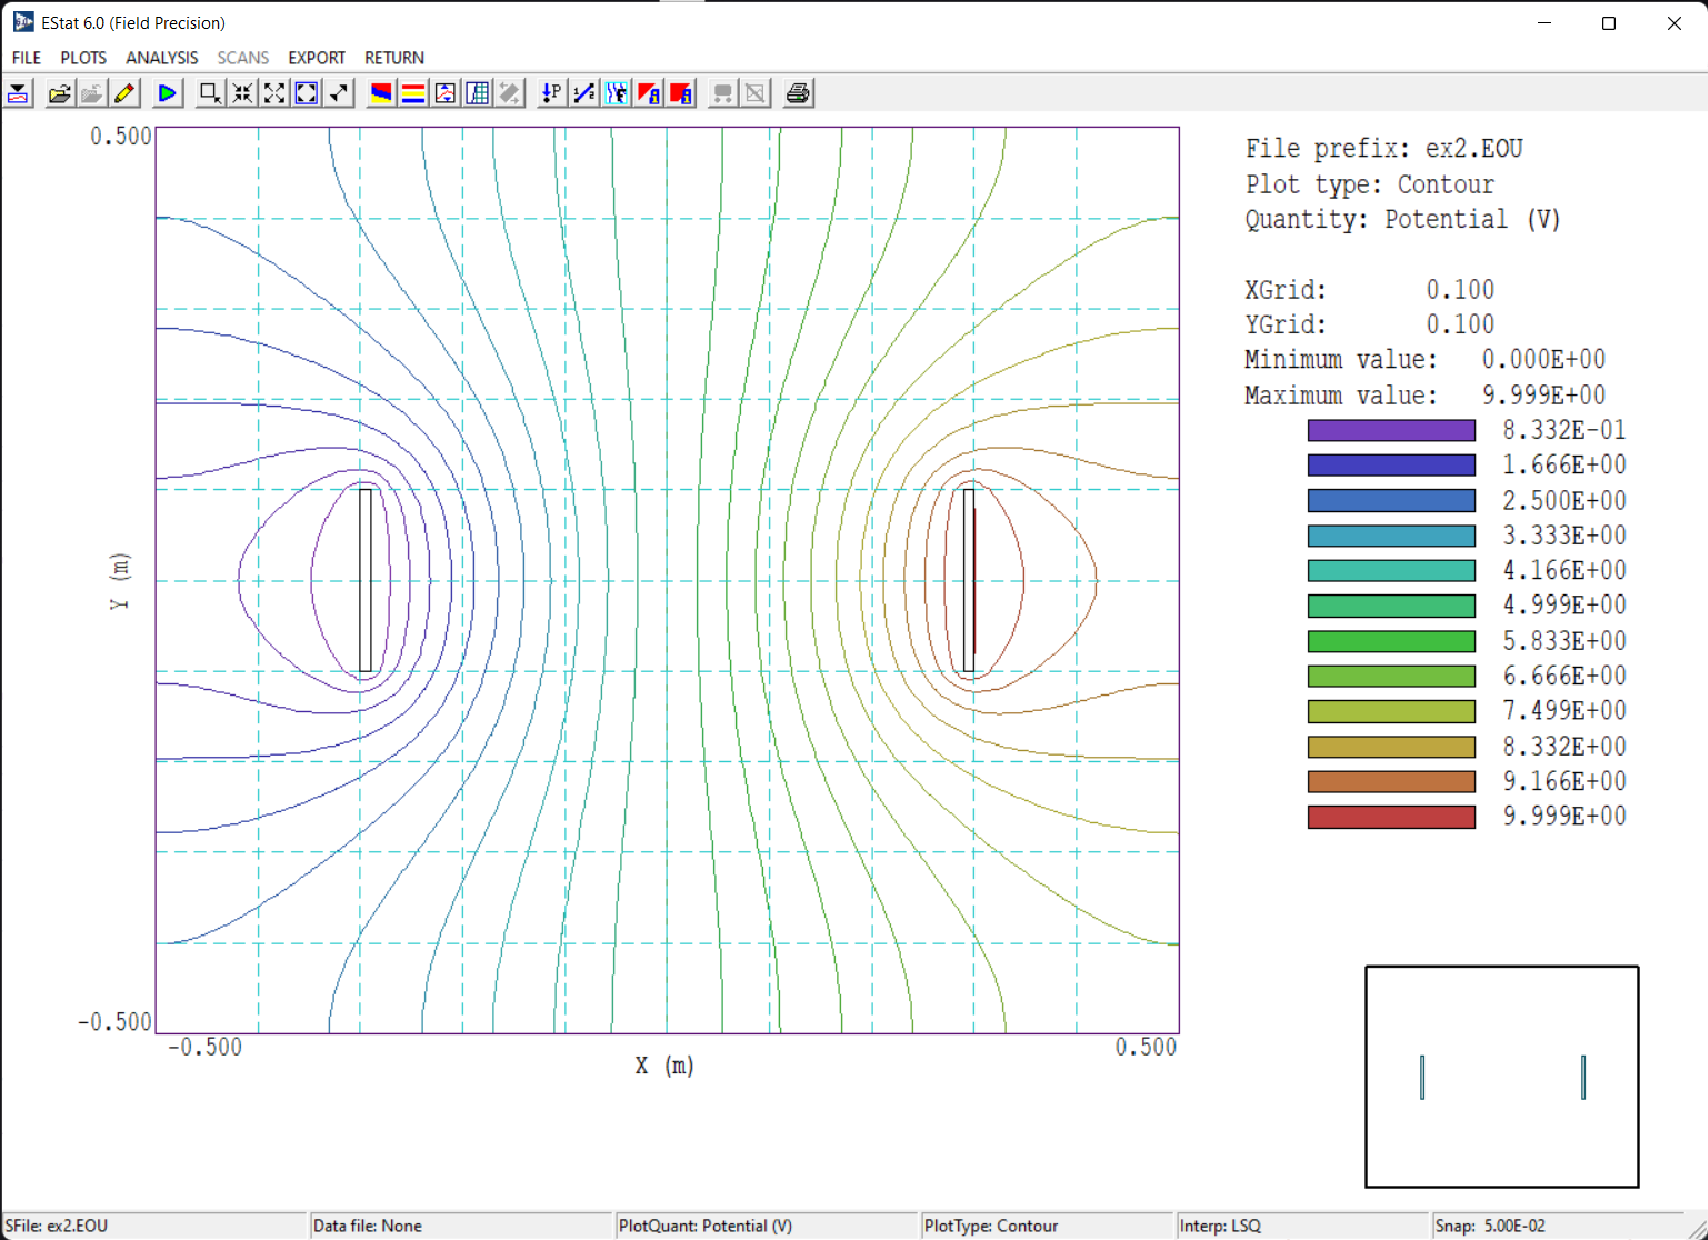
\includegraphics[scale=0.5]{figure2.pdf}
        \caption{境界が無限遠とした場合の等電位面}
    \end{center}
\end{figure}
\newpage

\subsection{実験課題3}
シミュレーション結果を以下の図3に示す.$x$座標が正の電極板に$10\,[\si{\volt}]$
の印加電圧がかかっており,$x$座標が負の電極板はGNDに接続しているとする.
\begin{figure}[H]
    \begin{center}
        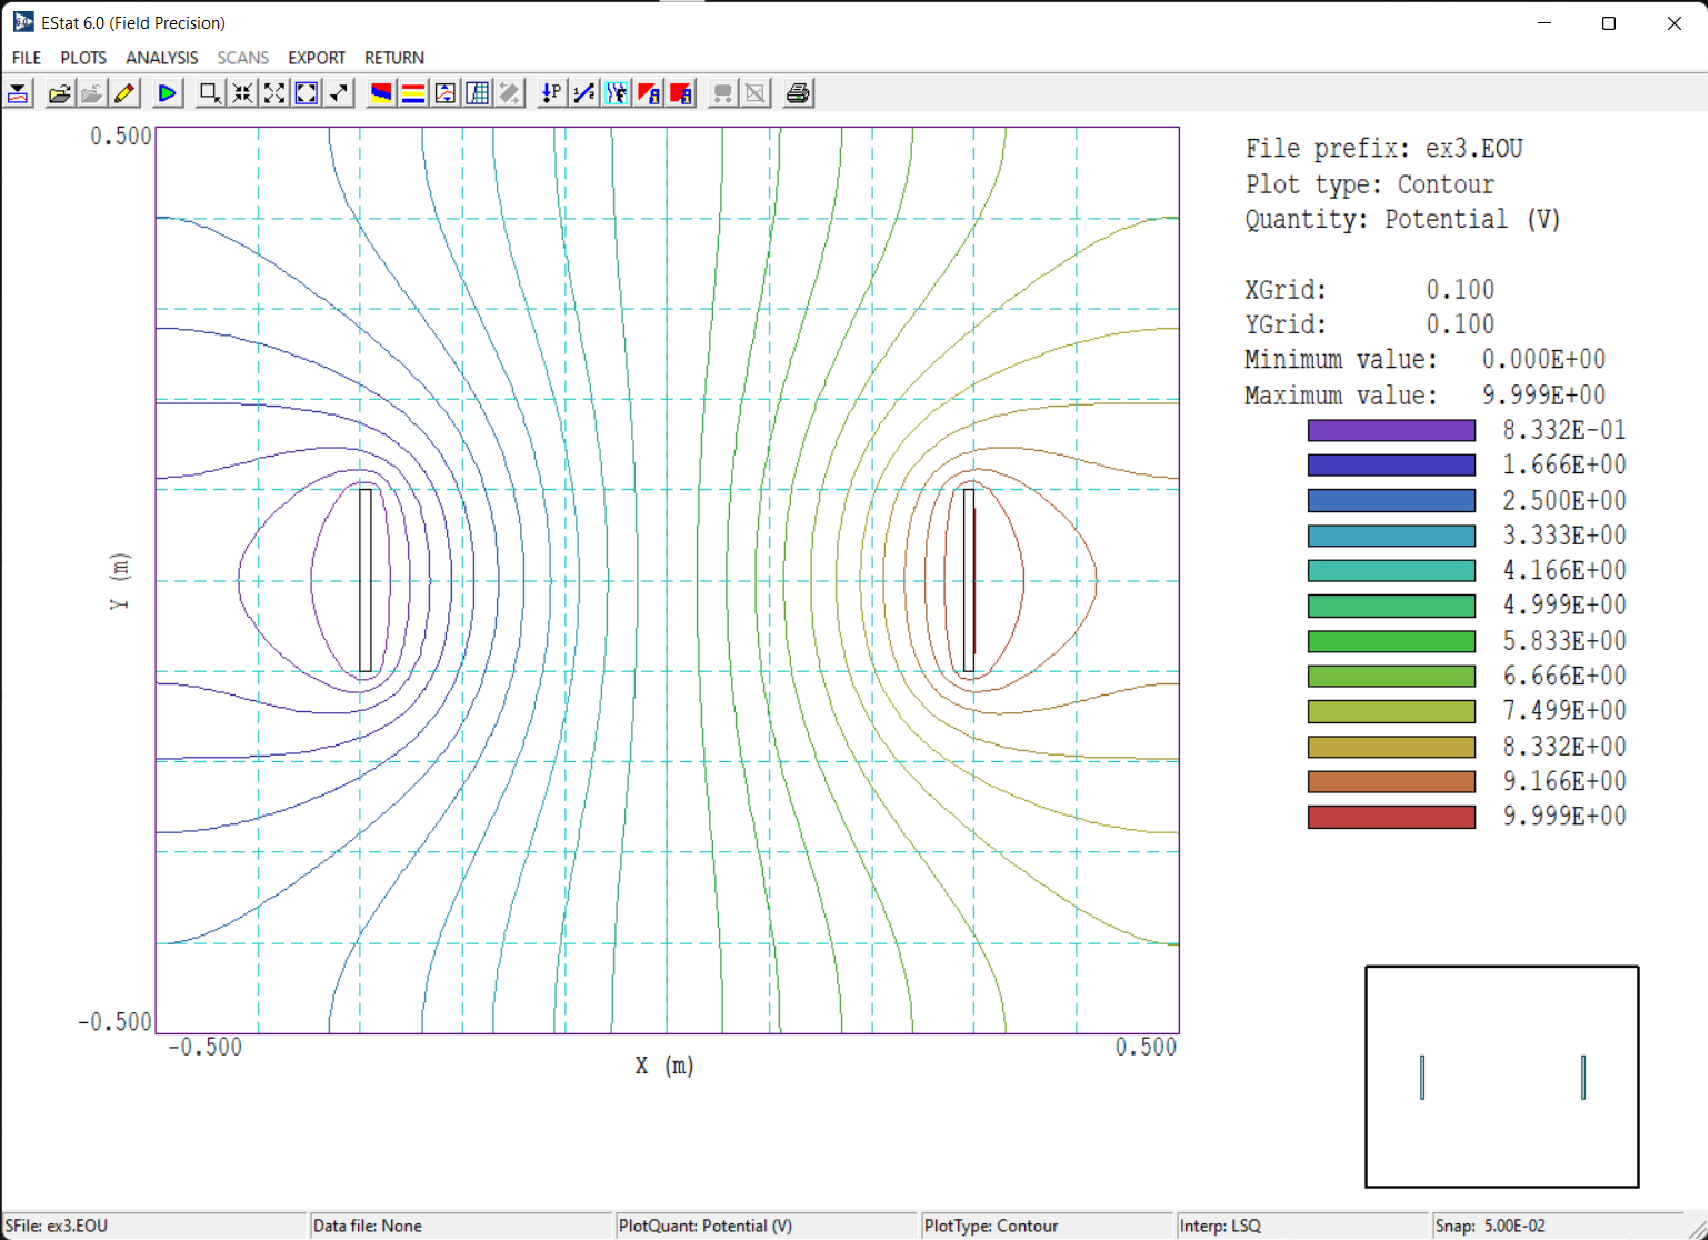
\includegraphics[scale=0.5]{figure3.pdf}
        \caption{媒質が真空の場合の等電位面}
    \end{center}
\end{figure}
\newpage

\subsection{実験課題4}
シミュレーション結果を以下の図4に示す.$x$座標が正の電極板に$10\,[\si{\volt}]$
の印加電圧がかかっており,$x$座標が負の電極板はGNDに接続しているとする.
\begin{figure}[H]
    \begin{center}
        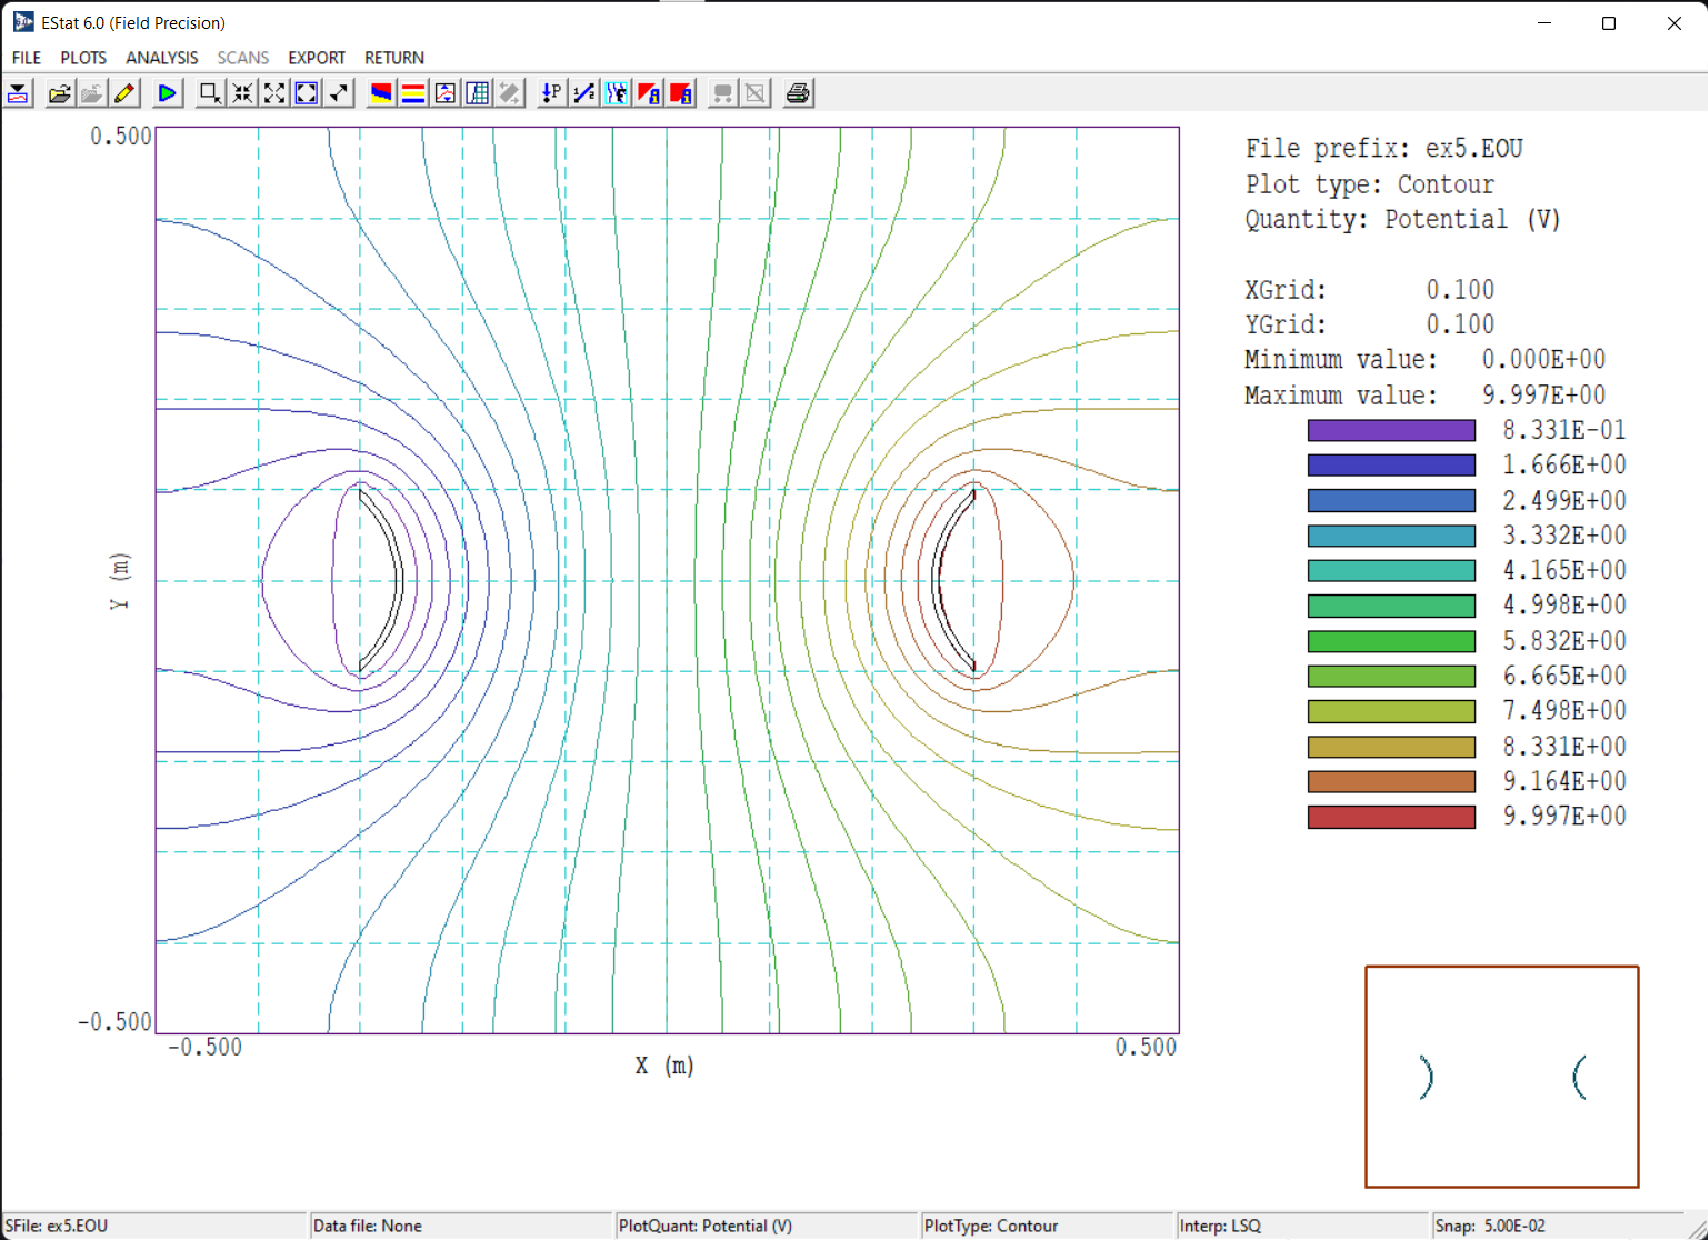
\includegraphics[scale=0.5]{figure4.pdf}
        \caption{電極板が曲面板の場合の等電位面}
    \end{center}
\end{figure}
\newpage